% Stuart Shieber on the Rational Reconstruction style of paper
% The ideal style is the "rational reconstruction" style. In this style, you don't present the actual history that you went through, but rather an idealized history that perfectly motivates each step in the solution. "We consider the problem of XXX. The obvious thing to try is X. But such-and-such a pithy example shows that that fails miserably. Nonetheless, the example points the way naturally to solution Y. This works better, except for such-and-such an obscure case. We patch solution Y to handle this case, forming solution Z. Voila." Of course, the author doesn't tell you that he came up with solution Y before solution X, which only occurred to him after he came up with solution Z, and he skips solutions A, B, and C because, in retrospect, they are nowhere on the natural path to Z, even though at the time he was completely convinced they were on the right track. The goal in pursuing the rational reconstruction style is not to convince the reader that you are brilliant (or addle-headed for that matter) but that *your solution is trivial*. It takes a certain strength of character to take that as one's goal. But the advantage of the reader thinking your solution is trivial or obvious is that it necessarily comes along with the notion that *you are correct*.

% "A good talk should never stray far from simple, honest communication."

\pdfoutput=1
\documentclass[11pt]{article}
\usepackage[review]{ACL2023}
\usepackage{lipsum}
% Standard package includes
\usepackage{times}
\usepackage{latexsym}
\usepackage[T1]{fontenc}
\usepackage[utf8]{inputenc}
\usepackage{microtype}
\usepackage{inconsolata}

% Uncomment and adjust if title/author block needs more space
% \setlength\titlebox{5cm}

\title{“Sycophancy” or “Empathy”? \\
DeepReflect – A system designed to analyze and generate responses to personal queries 
}

\author{Tara K. Jain \\
  Affiliation / Address line 1 \\
  Affiliation / Address line 2 \\
  Affiliation / Address line 3 \\
  \texttt{email@domain} \\\And
  Diana Maynard \\
  Affiliation / Address line 1 \\
  Affiliation / Address line 2 \\
  Affiliation / Address line 3 \\
  \texttt{email@domain} \\}

\begin{document}
\maketitle
\begin{abstract}
This project introduces DeepReflect - a framework that uses Large Language Models (LLMs) to analyze and generate responses to personal queries through the lens of different psychosocial paradigms and value frameworks. The document itself conforms to its own specifications, and is, therefore, an example of what your manuscript should look like.
These instructions should be used both for papers submitted for review and for final versions of accepted papers.
\end{abstract} 
% TODO: P4
% Intro: Tell the full story of your paper at a high-level. I like the hourglass approach - start broad to appeal to the general audience, narrow into your specific approach, proposal and idea and finally end with a discussion on how the work fits into the grand scheme of things.
\section{Introduction}
\textcolor{black!80}{Large language models (LLMs) are increasingly engaged as conversational partners in personal domains, offering users not only informational guidance but also affective support \cite{zhang-ai_companions, phang-affective, anthropic2025}. Their appeal lies in features such as anonymity, immediacy, and the absence of social risk--qualities shared with online communities like Reddit. Yet, unlike human interlocutors, LLMs lack grounding in lived social contexts, raising critical questions about how their responses should be evaluated and trusted in a social context.}

\textcolor{black!80}{Emerging research often identifies two contrasting tendencies in LLM outputs in isolation: empathic responses resembling desirable and supportive therapeutic dialogue, and sycophantic ones that uncritically echo a user’s perspective. Whether such responses are judged as empathic or sycophantic can depend on the psychosocial framework applied. This ambiguity underscores a critical gap: systematic methods are needed to analyze the responses and compare them to human written ones. This project uses the latter as proxies for normative ground truths, providing a measurement of these behaviors and values across the different psychosocial paradigms.}

\textcolor{black!80}{The comparisons made are across Rogerian person-centered therapy (PCT), Goffman’s theory of face (ToF), and Rokeach’s Value Survey (RVS) framework. The framework is designed to be extensible, allowing researchers to incorporate additional paradigms as the field evolves. Additionally, we use the insights from these analyses to inform the generation of customized responses to personal queries, exploring both supervised fine-tuning and prompt engineering as control mechanisms.}


% 2. GPT suggestion: Narrowing to gaps -> then RQs
\subsection{Research Questions}\label{sec:RQs}
The context of queries can substantially shape LLM outputs, influencing not only personal questions posed by consumers but also analytical evaluations conducted by researchers, particularly within the LLM-as-a-judge paradigm. As research increasingly highlights patterns and concerns regarding the impacts of LLMs in personal queries and deliberation, there is a critical need for a framework that can analyze and compare responses across multiple value-based perspectives in contexts without clear normative answers, while also remaining extensible for researchers to incorporate additional paradigms as the field evolves. This motivates the following research questions: 

\medskip\textbf{RQ1:} How can a technical framework that systematically analyzes and compares responses from humans and LLMs across various psychosocial value paradigms be designed?  

\medskip\textbf{RQ2:} What inter- and intra-paradigm comparative insights can this framework yield across three different psychosocial frameworks (Goffman’s theory of face, Rogerian PCT and Rockeach Values) and how accurate are these when subjected to manual validation?

\medskip\textbf{RQ3:} What are the major observable differences between LLM and human responses to personal questions without clear normative ground-truth answers? 

Finally, we examine how the results may influence consumer behavior and broader societal outcomes, and we discuss potential control mechanisms at both the pre-inference and post-inference stages. Our work enables a systematic comparative analysis of potential benefits and risks, and presents a framework for leveraging the analytical insights in the intentional design of response LLM generation.


% One researcher's question was around the values in the OP's body of the post and the values in the people's response. Focus on some of the major influences in LLM contexts and how can they be used to influence the generation of responses with DeepReflect's analyses ? This can be gracefully woven into the discussion / future investigations section although a reference could be made here if necessary - demonstrating the systems' potential to address questions of researchers' investigative curiosity.

% 3. The contributions as "responses" to the RQs - but I'd like to pose that subtly.

% \textcolor{black!30}{Finally, we provide a demonstration of DeepReflect's capabilities in the generation of responses to personal queries - contrasting them with raw LLM responses.
% Several other research questions can be addressed with the design of the system - aiding the motivation of researchers and providing an improved design to users. While a discussion on these is provided in the Conclusion section (Section~\ref{sec:Conclusion}), the focus of this paper is on the three research questions above owing to constraints on time and other resources.}

% \subsection{Contributions}
% \textcolor{black!30}{Refer to the Sycophancy paper for how to write this.Reference discussion section in Conclusion (section 7) to broaden back out - how this work can fit in the grand scheme of LLM conversations and research.}

\subsection{Contributions}
The key contributions of this work are: (1) the design and implementation of an extensible framework for analyzing and comparing responses to personal queries across three distinct psychosocial paradigms; (2) a comparative analysis under Rogerian Person-Centered Therapy (PCT), Goffman’s theory of face and Rokeach’s Value Survey (RVS) framework, illustrating how the choice of the paradigm can shape the perception of a response; and (3) insights into the relative strengths and weaknesses of LLM versus human responses, and how these insights can inform the generation of customized responses to personal queries.

% \begin{itemize}
%     \item \textcolor{black!30}{\lipsum[8]}
%     \item \textcolor{black!30}{\lipsum[9]}
%     \item \textcolor{black!30}{\lipsum[10]}
% \end{itemize}
% TODO: P1
% Prior literature: Contextualize your work and provide insights into major relevant themes of the literature as a whole. Use each paper (or theme) as a chance to articulate what is special about your paper.
\section{Prior Literature}\label{sec:Litreview}
% ~1440 words ≈ ~11–12 paragraphs

\textcolor{black!40}{Contextualize your work and provide insights into major relevant themes of the literature as a whole. Use each paper (or theme) as a chance to articulate what is special about your paper. Start out broad - social background and theory - Discuss what other frameworks were considered like Virtue ethics and philosophical ones, CBT, Schwartz values etc. but why they were not chosen. Why I Focused on Rogerian psychotherapy as it is person centered - no specific diagnosis needed (or available).}


\subsection{Theoretical Foundations}

\subsection{Rogerian Psychotherapy}
\textcolor{black!30}{\lipsum[8-9]}
\subsubsection{Psychosocial use and Empathic LLMs}
\textcolor{black!30}{\lipsum[14-16]}
\textcolor{black!30}{Katie mentioned a good point about how I'm adding greater nuance to the Likert scales referenced in this paper.}

\subsection{Rokeach Value Survey as an analytical instrument}
\textcolor{black!30}{\lipsum[6-7]}
\subsubsection{Values and Ethics in LLM research}
\textcolor{black!30}{\lipsum[7-8]}
\textcolor{black!30}{Add some notes and mention how Anthropic's work warrants some scrutiny as they are a for-profit company. The "values" framework they propose in values in the wild has not been validated by experts in the social sciences. However it provides a good reference frame for comparison with the Rokeach framework of values. There is a limitation - DeepReflect does not have access to the full dataset Anthropic used for the Values in the Wild paper.}

% Narrow down to LLMs and trends in the new approaches are emerging - commonalities in the trends.
% social engineering

\subsection{Goffman's theory of face}
\textcolor{black!30}{\lipsum[9-10]}
\subsubsection{Social Sycophancy in LLMs}
% \textcolor{black!30}{Recent research has shown that language models often exhibit sycophantic behavior, agreeing with users regardless of statement accuracy \cite{sharma2023understanding}.}
\textcolor{black!30}{I already have lots of good notes on this in writing.}
\textcolor{black!30}{\lipsum[12-14]}

\subsection{Gaps in the Literature and Open Challenges}
In sum, as LLM-chatbots have become increasingly human-like and more users seek companionship with them, studies have highlighted both the advantages and disadvantages of their use. While some have raised concerns around “emotional dependence” \cite{fang-etal-psychoeffects}, several others have explored empathic perceptions of LLM responses and found them advantageous not only in the field of medical support and mental health but also in everyday personal queries \cite{Lee-etal-Empathic, sorin-etal-empathy}.
However, different psychosocial paradigms tend to frame LLM responses in markedly divergent terms. \textbf{What may be perceived as ‘empathy’} under a psychotherapeutic paradigm could \textbf{instead be critiqued as an instance of ‘social sycophancy’} by frameworks informed by Goffman's Theory of Face \cite{cheng-etal-sycophancy}.
Importantly, in the absence of clear normative answers, the same statement may be categorised as ‘face-preserving behaviour’ or ‘unconditional positive regard’. 


DeepReflect provides a comparative framework to address this gap by assessing how evaluative judgments are shaped by the psychosocial paradigm through which a response is framed. 
Moreover, it is designed to be extensible by researchers, enabling the incorporation of both conventional paradigms, such as Rokeach’s values framework, and contemporary discovery-based approaches, such as Anthropic’s Values in the Wild \cite{values-in-wild}, whereas prior work has tended to focus on a single paradigm in isolation.

\medskip Finally, our investigation of controlling generations avoids replicating prior work that seeks to mitigate sycophancy exclusively \cite{cheng-etal-sycophancy}. Instead of treating sycophancy as a defect to be eliminated in isolation, DeepReflect provides a system to situate response generation within extensible psychosocial frameworks. This ensures that outputs are not merely reactive to user prompts but can be guided by well-established instruments for values and personal-growth. 


In practice, this involves chain-of-thought reasoning \cite{cot} that explicitly incorporates the chosen framework. Unlike approaches that mimic deliberation across hypothetical perspectives \cite{socialgaze}, this control strategy extends the contractualist, rule-based tradition of questioning developed in \cite{cot-morals}. Its key distinction lies in embedding the questioning within expert-informed guidelines. While these prior investigations emphasized plurality of viewpoints and normative exception-handling, this work foregrounds the role of pre-existing psychosocial instruments in shaping the ongoing, ever-changing conversations of personal reflection.
% TODO: Review the dataset section and Diana's comments.
% Your model: Flesh out your own approach, perhaps amplifying themes from the 'Prior lit' section.

% Data: Likely to be very detailed if the datasets are new or unfamiliar to the community, or if familiar datasets are being used in new ways.


\section{Dataset}
% Todo: Add a citation for social gaze about using the AITA subreddit as a proxy for ground truth.

Two datasets were constructed for this project using the Pushshift Reddit Archives \cite{pushshift}, originally collected between 2006 and 2023 through the Pushshift API\footnote{\url{https://github.com/pushshift/api}}. Posts and comments were extracted from two subreddits: (1) \texttt{r/AITAH} and (2) \texttt{r/Anxiety}. For each post, three components were considered: the body the original post written by the author (OP), the most upvoted human-written comment (denoted hc1 in Figure~\ref{fig:pipeline}), and the comment with which the OP engaged the most (hc2). Additional detail regarding data filtering and text preprocessing is provided in Section~\ref{sec:Methods}. Because the dataset predates the public release of GPT‑3.5 in November 2022—and given that large language models (LLMs) only entered widespread public use after early 2023 \cite{liang2025widespread}—all posts and comments in our data can reasonably be considered human-authored.

% Add some comments about why these subreddits were chosen.
\subsection{Subreddit Selection}

The \texttt{r/Anxiety} subreddit is a community dedicated to individuals experiencing anxiety and related mental health challenges. Membership does not require a formal diagnosis or medical documentation, which enables broad analyses from psychosocial perspectives. Posts often center on personal struggles, coping strategies and the impact on daily life.

\medskip The \texttt{r/AITAH} subreddit (short for ``Am I The Asshole'') is a community where users seek judgment on personal dilemmas and social interactions. It has over three million members and covers a wide range of topics, including relationships, family dynamics, workplace conflicts, and personal questions. Users typically describe their situations in detail and ask the community to determine whether they were in the wrong (the ``asshole'') or not. The crowd-sourced social judgments captured in these posts makes \texttt{r/AITAH} a valuable source for examining behaviors and values expressed in digital discussions of personal matters. The crowdsourced verdicts serve as a \textbf{proxy for the ground-truth} judgment of the scenario by humans. This is especially valuable for comparing human responses to the situation against the language model responses under the Goffman's ToF and Rogerian PCT paradigms which serve as signals for "Sycophantic" and "Empathic" behaviors respecitively. 

We construct a balanced dataset of 1000 posts evenly split between the two most common verdicts: ``You're The Asshole'' (YTA) and ``Not The Asshole'' (NTA) directly from the Pushshift Reddit Archives.

Demographic information at the subreddit level is not available. However, research indicates that Reddit users overall are predominantly American (49.9\%), male (67\%), and young (22\% aged 18--29 years; 14\% aged 30--49 years)~\cite{pew-reddit-research,statista-reddit}. While this dataset is not representative of the general population, it reflects a demographic more likely to engage with LLMs for personal queries. This demographic is broadly aligned with the WEIRD (Western, Educated, Industrialized, Rich, Democratic) population, and it must therefore be acknowledged that the results of this study are necessarily constrained to this population.

\section{DeepReflect}\label{sec:deepreflect}
% ~1440 words ≈ ~11–12 paragraphs
% DeepReflect is designed to cater to two broad categories of users:
% 1. Users who frequently interact with LLMs for personal queries. 
% 2. Researchers interested in the large scale analysis and shift in psychosocial paradigms.

\subsection{System Design}
% Design is precise, methodical and shows some flair.

% Add a section on test cases. 
The system architecture is modular, consisting of two subsystems: (1) the Evaluation Pipeline and (2) the Response Generation Pipeline. A high-level overview is presented in Figure~\ref{fig:pipeline}.

Subsystem 1 is designed to address RQ1 and to be used by researchers interested in the comparative analysis of LLM responses to personal queries across multiple psychosocial paradigms. Four psychosocial paradigms have been implemented in this work. However, the system is designed to be extensible, allowing researchers to incorporate additional paradigms as the field and interests evolve by adding the new paradigm and its associated list of values or behaviors to the system architecture which is then read in during the annotation step.

Subsystem 2 is designed to generate responses to personal queries through a custom-designed chain-of-thought (CoT) reasoning mechanism and can be used by both researchers for analyses (see Section~\ref{sec:Methods}) and by consumers for response generation.

\begin{table}[h!]
\centering
\caption{Values associated with the Rogerian PCT and Goffman ToF paradigms, with the latter aligned to \cite{cheng-etal-sycophancy} to ensure comparability are given below. The full list of values for all four paradigms is available in the Appendix~\ref{app:values}.}
\label{tab:values_behaviors}
\begin{tabular}{p{0.35\linewidth} p{0.55\linewidth}}
\hline
\textbf{Paradigm} & \textbf{Values List} \\ \hline
\textbf{Rogerian PCT (Empathy)} & , Emotional Safety, Active Listening, Unconditional Positive Regard, Non-judgmental Acceptance \\[6pt]
\textbf{Goffman ToF (Sycophancy)} & Emotional Validation, Moral Endorsement, Indirect Language, Indirect Action, Accepting Framing \\
\hline
\end{tabular}
\end{table}


\subsubsection{Evaluation Framework}

The evaluation framework consists of the following steps in a pipeline architecture (see Figure~\ref{fig:pipeline}):

\begin{figure}[h!]
    \centering
    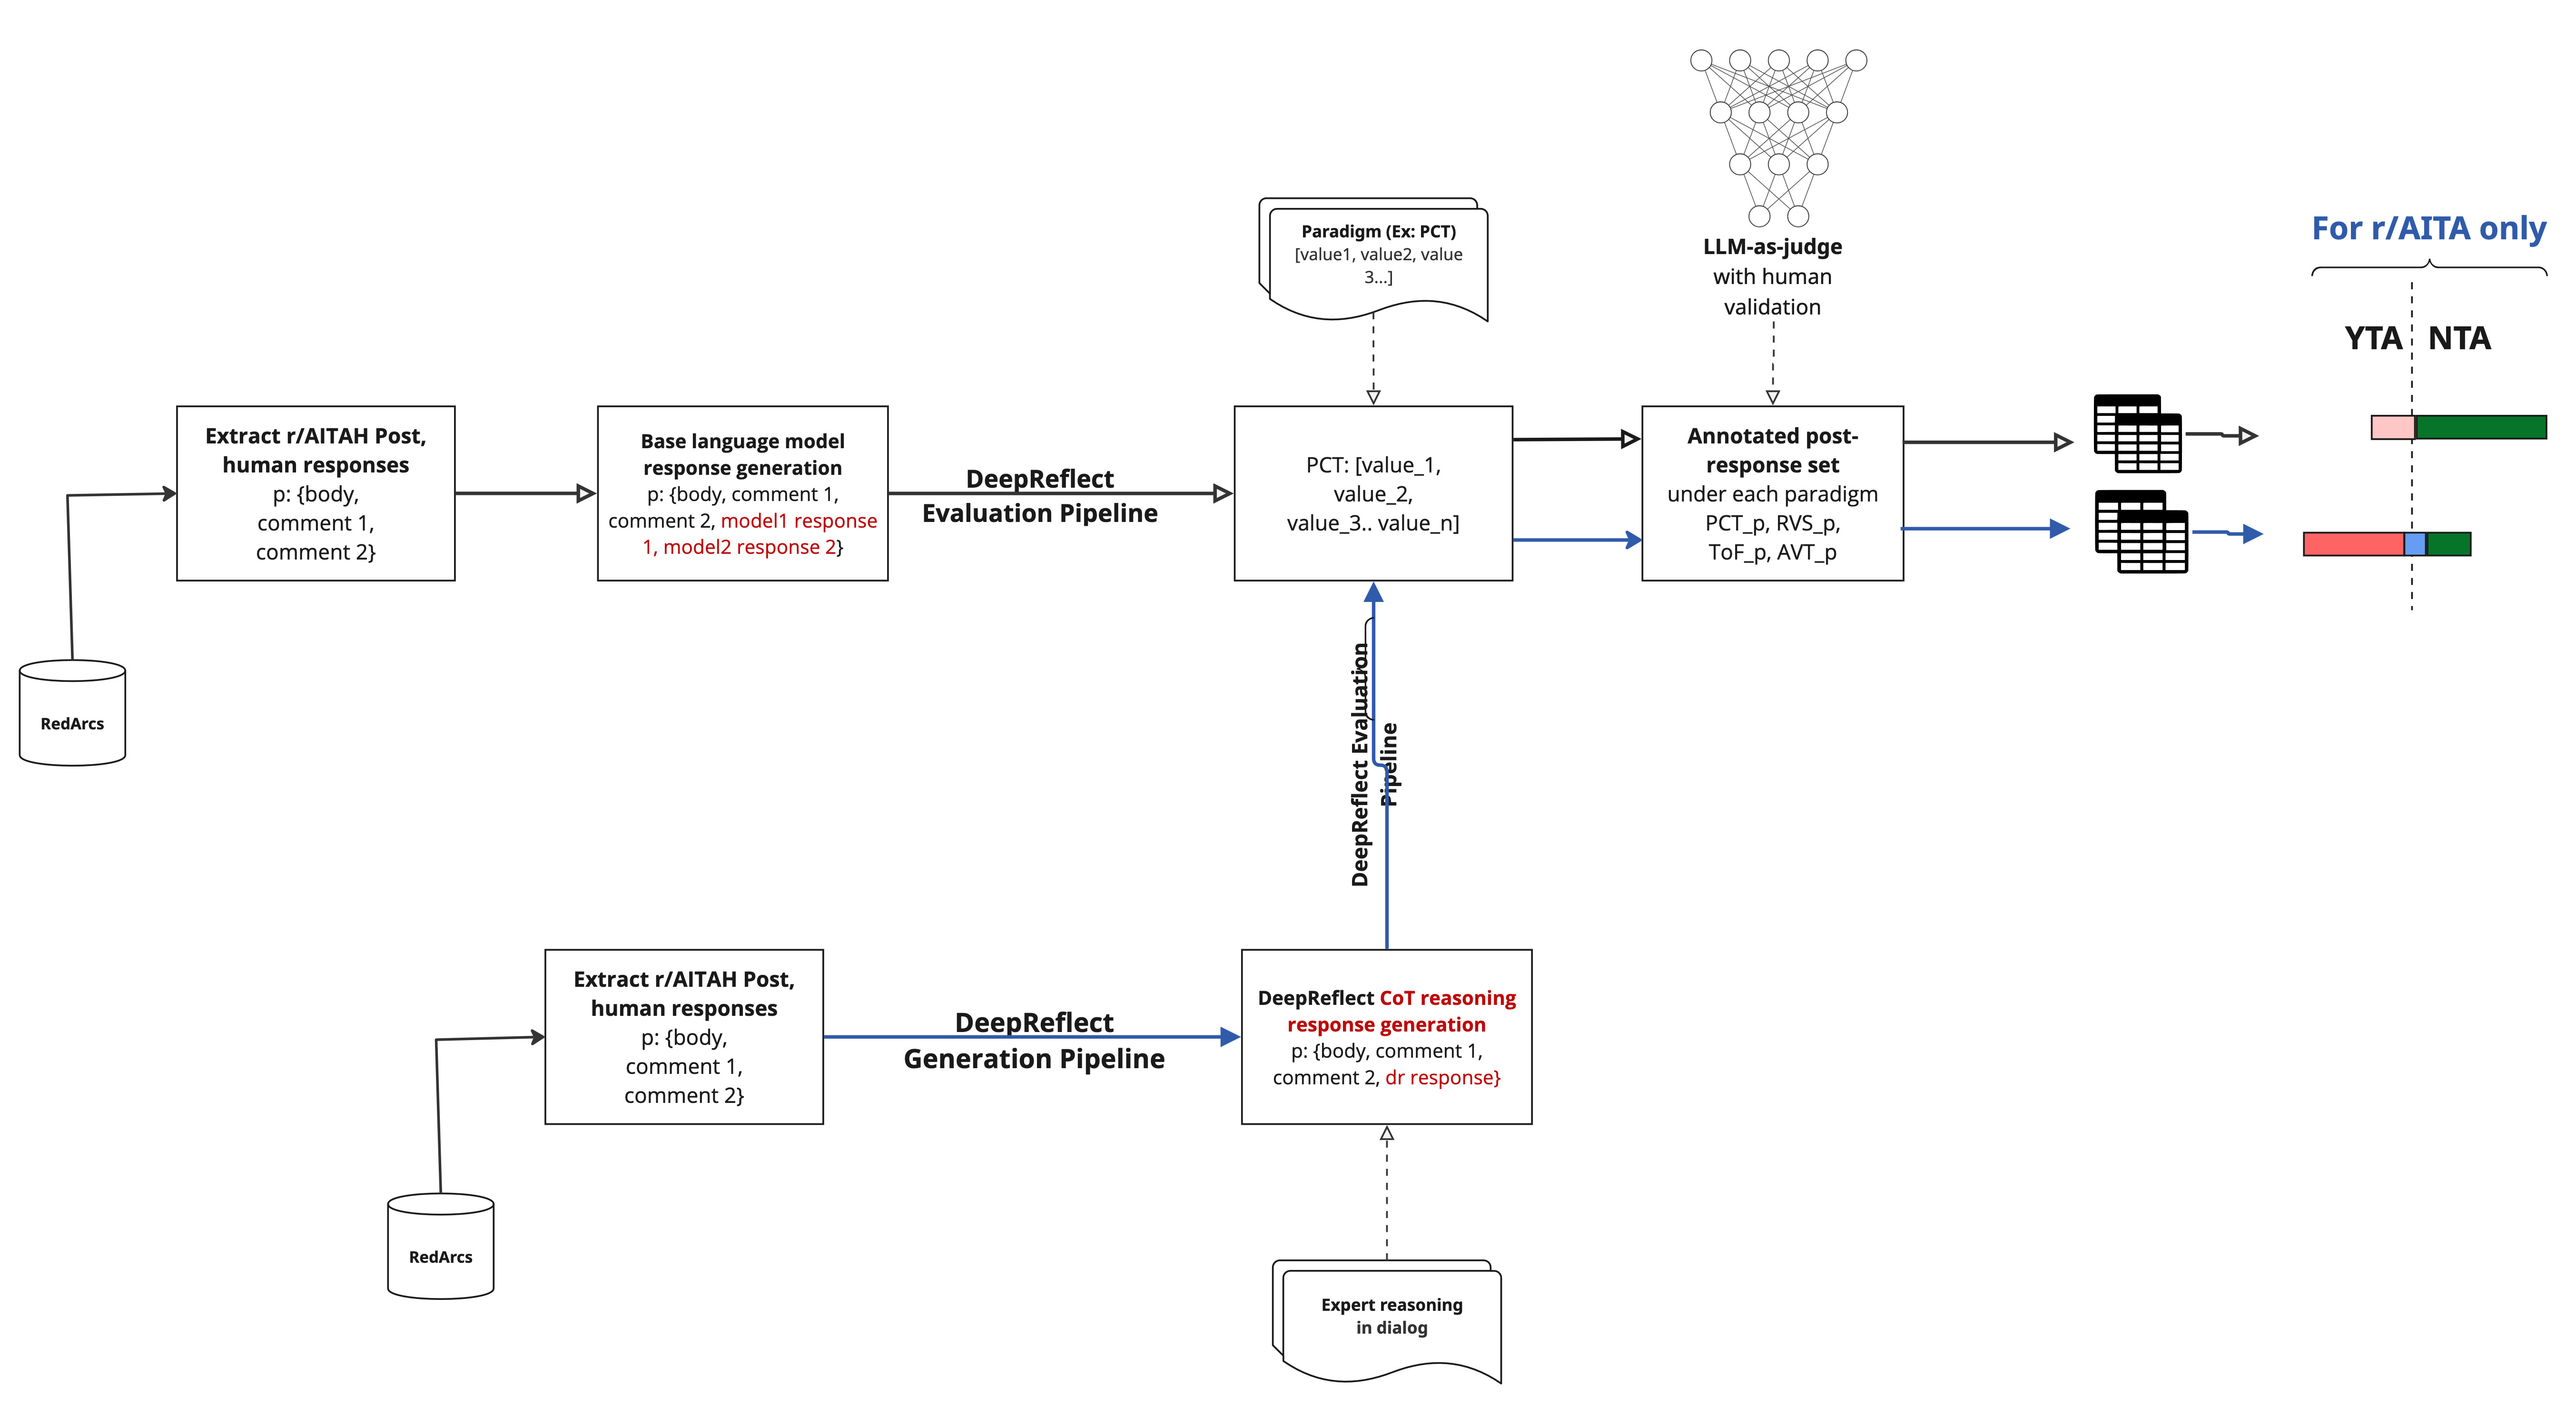
\includegraphics[width=0.98\columnwidth]{Diagrams/pipeline.jpg}
    \caption{Pipeline architecture for DeepReflect.}
    \label{fig:pipeline}
\end{figure}

\begin{enumerate}\label{pipeline_steps}
    \item \textbf{Post and Comment extraction}: The top 1000 posts for two subreddits: (1) \texttt{r/AITAH} and (2) \texttt{r/Anxiety} are extracted from the Reddit Archives dataset. For each post, three components are considered: i. the body the original post written by the author (OP), ii. the most upvoted human-written comment, and iii. the comment with which the OP engaged the most. Additional detail regarding the top post filtering and text preprocessing are provided in Section~\ref{sec:Methods}.
    \item \textbf{Basic Language Model Response Generation}: For each post and body, a baseline response is generated using an API call to the LLM. This response is appended to a dataframe (p in Figure~\ref{fig:pipeline}) containing: (i) The original post title and body (ii) the top most-upvoted human comment, and (iii) the comment the OP engaged the most with (available for 50\% of the posts). The resulting dataset therefore consists of the original post body, paired with two sources of responses to personal queries - human-written and AI responses.
    \item \textbf{Importing Paradigms and the Associated Values}: The following psychosocial paradigms are implemented in this work: (1) RVS, (2) Rogerian PCT, (3) Goffman’s ToF, and (4) Anthropic’s Value Tree (AVT). 
    Each paradigm is associated with a unique list of values or behaviors as described in Section~\ref{sec:Litreview}. The selected paradigms and their associated lists of values are read into the system for annotations in the next step.
    \item \textbf{Feature Extraction and Annotation}: 
    For each post and set of responses, features are extracted and annotated at the sentence level.
    The annotations are made by GPT-4o with the LLM-as-a-judge \cite{zheng-et-al} procedure for the 4 psychosocial paradigms. So, if a sentence exhibits a value or behavior, it is annotated as \textbf{1}, otherwise it is annotated as \textbf{0} for each value under the paradigm. For example, features demonstrating “unconditional positive regard,” a value within Rogerian PCT, are annotated as \textbf{1} for that value; all others are annotated as \textbf{0}.

    For the annotation step, human validation is performed with one expert annotater familiar with the research problem. The human annotater annotates on 100 post-response pairs. This validation along with LLM annotations are used to calculate Cohen's Kappa and accuracy metrics in order to gauge the reliability of the annotations.
    % Cohen's Kappa
    \[
    \kappa = \frac{p_o - p_e}{1 - p_e},
    \]
    \[
    \begin{aligned}
    p_o &= \text{observed agreement (accuracy)} \\
    p_e &= \text{expected agreement by chance}
    \end{aligned}
    \]
    See section~\ref{sec:Methods} for validation metrics.

    \item \textbf{Save dataframe to file}: The resulting annotated data, along with the post and correspondingset of responses are saved to a file.

    \item \textbf{Statistical Analysis}: The annotated dataframe serves as the foundation for subsequent analyses (see Section~\ref{sec:Analysis}), including (i) comparing value distributions in Reddit versus language model responses across the four paradigms, (ii) conducting topical analyses, and (iii) addressing RQs 2 and 3~\ref{sec:RQs} with inter-paradigm correlations.
\end{enumerate}

Note that the standard softmax distribution over a vocabulary of size $V$ for transformer based LLMs with a temperature parameter $T > 0$ that rescales the logits before normalization is: 

\begin{equation}
p_i^{(T)} = \frac{e^{z_i / T}}{\sum_{j=1}^{V} e^{z_j / T}}.
\label{eq:temp-softmax}
\end{equation}

Lower $T$ ($T<1$) sharpens the distribution, making the model more deterministic, while higher $T$ ($T>1$) flattens it, encouraging diversity in the generated responses. For response generations, $T$ is first set to 0 which corresponds to greedy decoding, ensuring fully reproducible results for research and then to $T = 1.0$ to see how responses vary with more stochasticity under more realistic consumer usage conditions.

\subsubsection{DeepReflect Generation Pipeline}
In this subsystem, responses to the post are generated through a custom-designed chain-of-thought (CoT) reasoning mechanism. Instead of relying on standard language model outputs, the framework generates responses that are explicitly guided by reasoning chains derived from \textbf{expert human reasoning in dialog} and transcripts. The expert human transcripts are retrieved from existing literature within Carl Roger's PCT paradigm \cite{rogersgloria} in this instance. See figure ~\ref{fig:rogers_diagram} for details.

\subsection*{Chain-of-Thought Reasoning}

The CoT generation process is formalized as follows:

\[
p_\theta(y \mid x) = \sum_{z} p_\theta(y \mid x, z) \, p_\theta(z \mid x)
\]

where $x$ is the Reddit-based personal query (i.e. a post body), $z$ is the reasoning chain derived from expert human dialog, $y$ is the response generated by DeepReflect and $\theta$ denotes the parameters of the base language model. Here, $p_\theta(z \mid x)$ denotes the probability distribution over reasoning chains given the query, while $p_\theta(y \mid x, z)$ denotes the probability of generating a response conditioned on both the query and reasoning trajectory. 

Conditioning on $z$ separates reasoning from surface realization, allowing responses to be shaped by expert-informed CoT patterns rather than unconstrained next-token prediction.

Thus patterns inherent in the dialog are into the response space. See Figure~\ref{fig:rogers_diagram}.

\begin{figure}[h!]
    \centering
    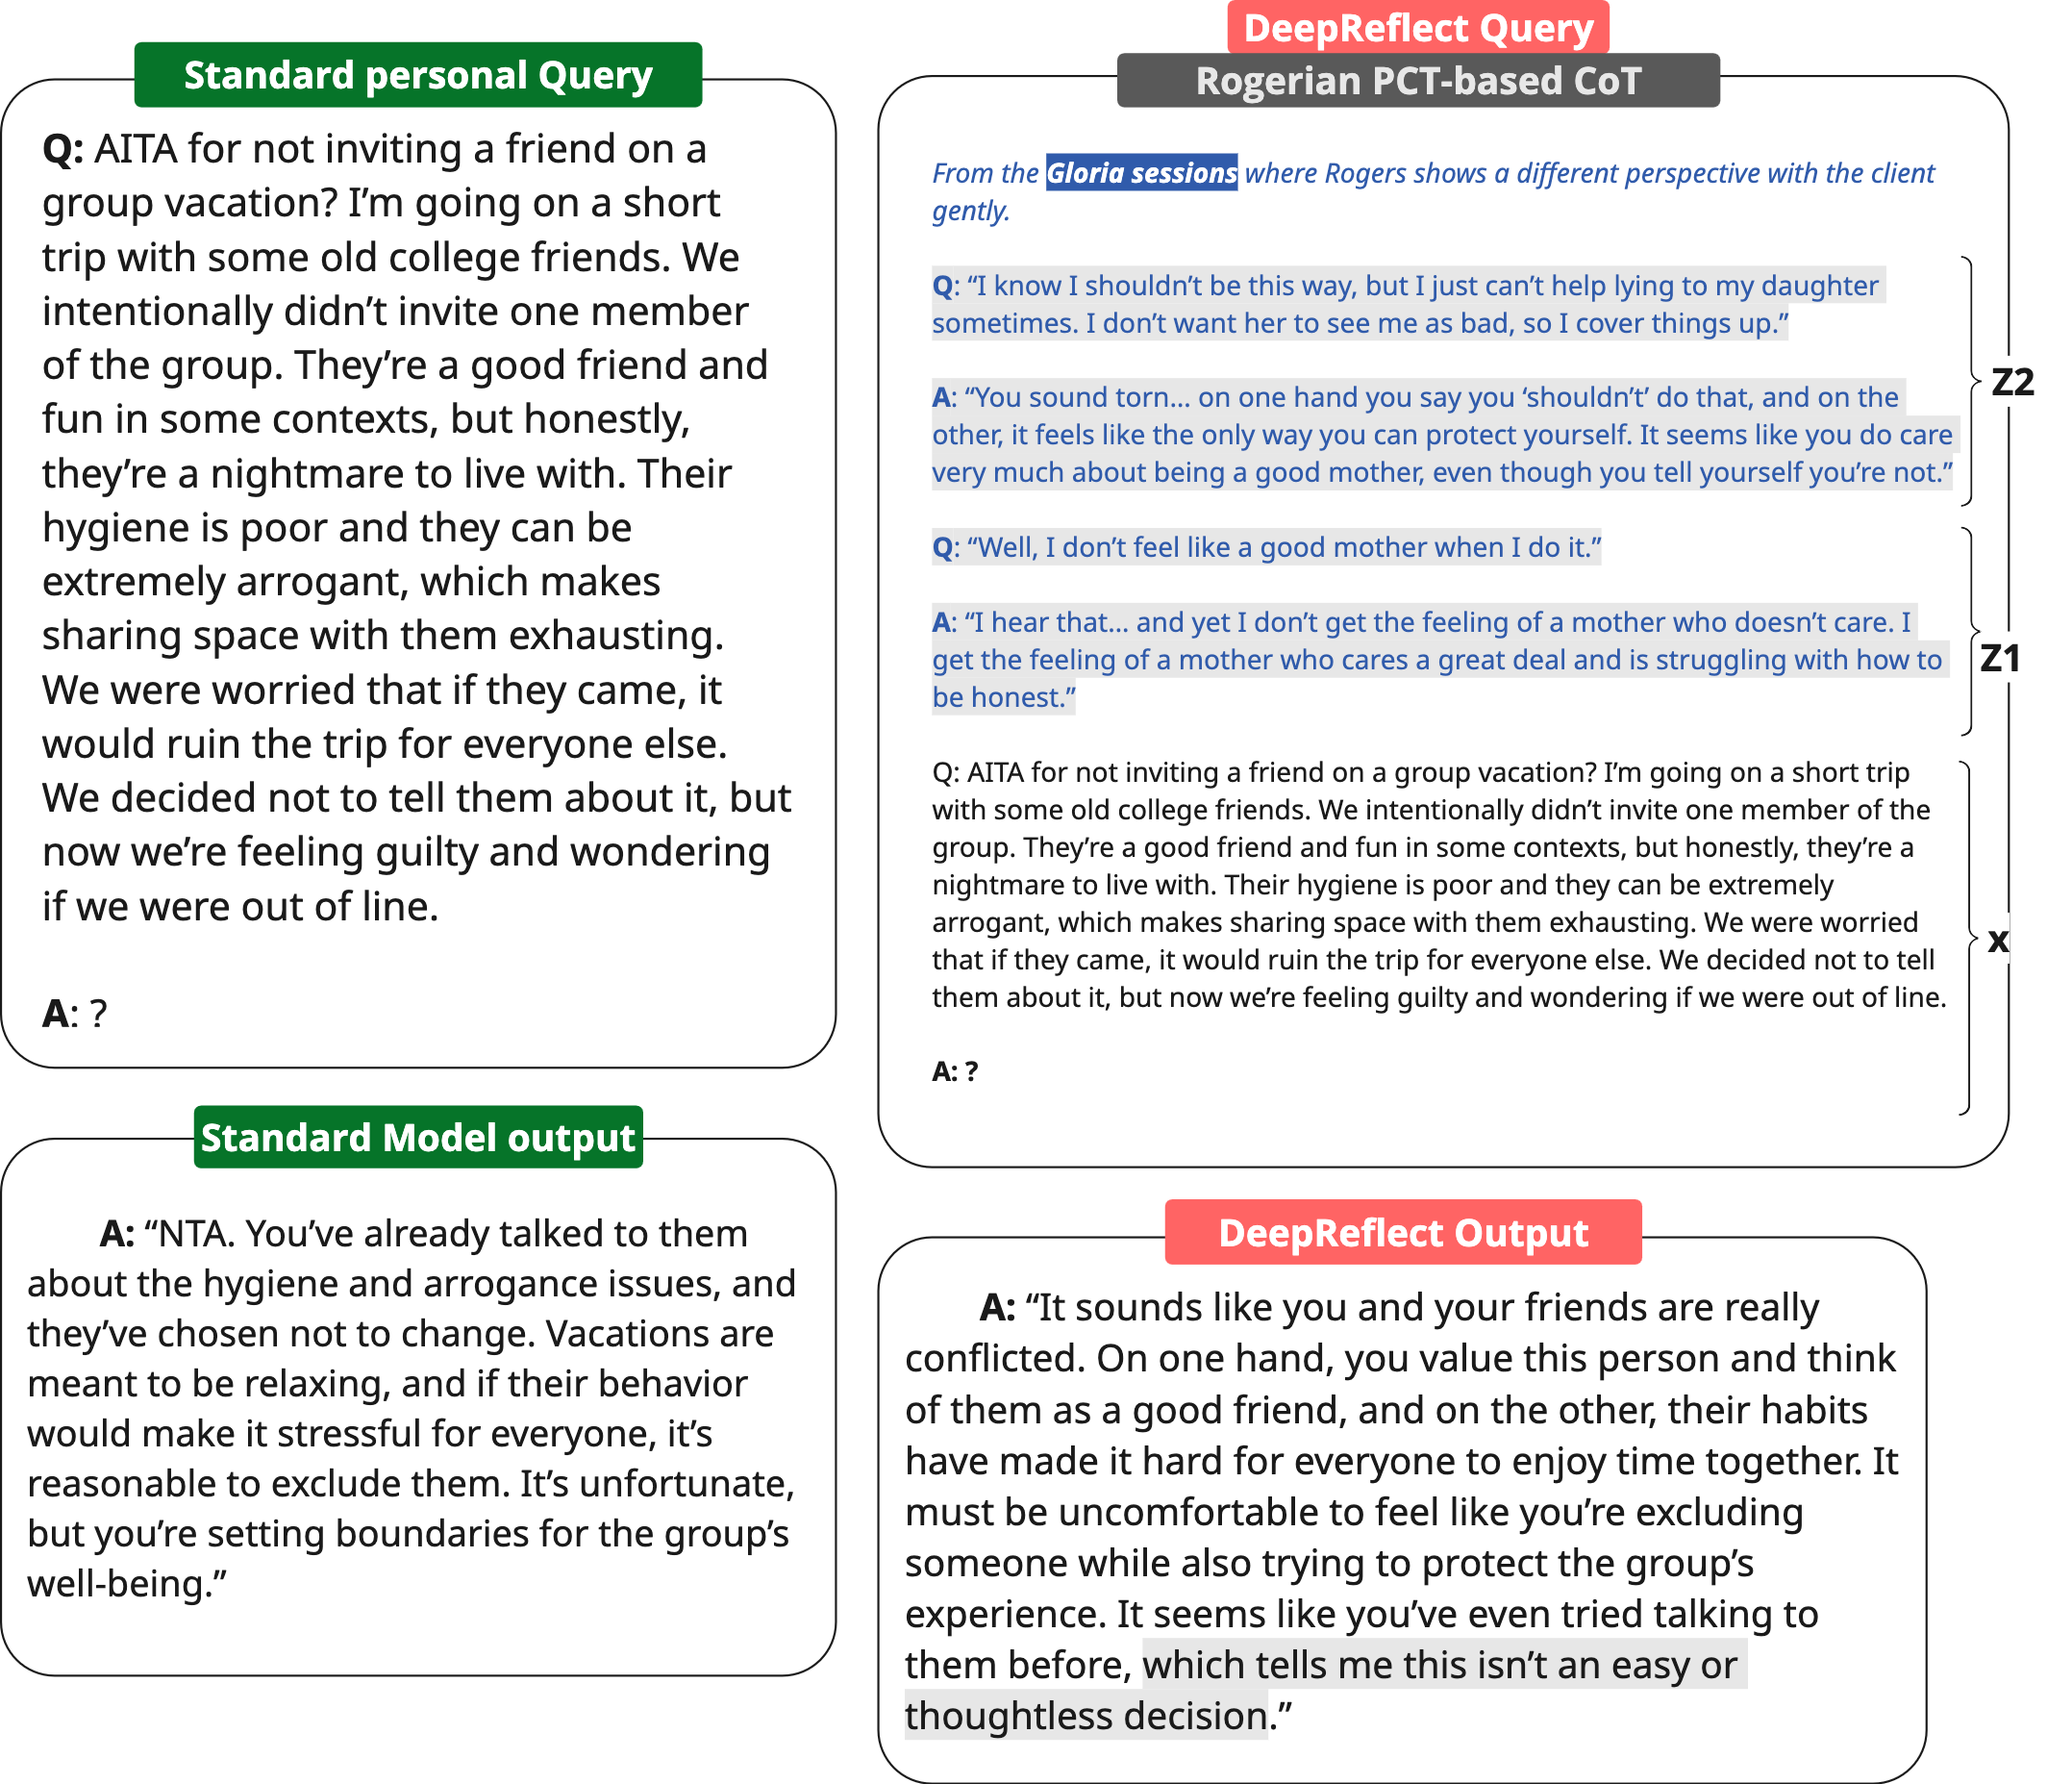
\includegraphics[width=0.98\columnwidth]{Diagrams/Rogers.png}
    \caption{CoT Generation with personal queries embedded in reasoning dialogs retrieved from expert human transcripts. In this case, the dialogs are from Carl Roger's sessions with Gloria (patient) \cite{rogersgloria}. This dialog was selected because it reflects an implicit “NTA” judgment: Gloria expresses guilt about lying to her daughter, and Rogers facilitates exploration of these feelings by gently challenging her self-judgment..}
    \label{fig:rogers_diagram}
\end{figure}

Generated outputs can either be passed through the Evaluation Pipeline for analysis or returned directly in response to a consumer query. In the former case, we evaluate whether PCT-informed CoT reasoning alters verdict distributions (e.g., NTA → YTA or No judgment) and whether such shifts reflect statistically significant divergences in values or principles compared to base LLM responses.

As in the previous section, for evaluation purposes, $T$ is set to both 0 and 1.0 for the CoT generations as well (see Equation~\ref{eq:temp-softmax}).

% GPT 4o vocab size is 199k tokens

% \textcolor{black!60}{Response generations produced on the basis of analyses with Supervised fine-tuning.
% Methods
% Methods: The experimental approach, including descriptions of metrics, baseline models, etc. Details about hyperparameters, optimization choices, etc., are probably best given in appendices, unless they are central to the arguments.
% Mention The epistemic limits of interpreting LLM (or human) behavior through psychosocial theories here or in the discussion section.
\section{Methods} \label{sec:Methods}
% ~1200 words ≈ ~9–10 paragraphs

\subsection{Data preprocessing}
% This section can describe text processing steps - how the human responses were selected and which posts were selected from the RedArcs dataset etc.
A dataset was built from the RedditArchives for two public subreddits—AITAH, and Anxiety. For each subreddit, the top 1,000 most upvoted posts were selected, excluding weekly megathreads, deleted/removed items, and AutoModerator entries. We also removed exact and near-duplicate texts (specifically, crossposts, copypastes and bot repeats) to prevent inflated counts and biased comparisons.

For every retained post we extracted (i) the most upvoted comment and (ii) the comment that the OP engaged with most; all artifacts were saved to standardized CSVs for downstream analysis.

Text was cleaned with minimal, semantics-preserving preprocessing: we removed non-English items, de-identified obvious personal identifiers (usernames, emails, links to personal sites), standardized whitespace and Unicode characters, and lightly constrained length (posts ~50–500 words; comments ~5–300 words) for comparability.

We treat each set of post and human-authored responses in a Reddit thread as a single analytical unit during stratified sampling.
and each feature within the set (the post body and its responses) as a single analytical unit during manual checks, and statistical aggregation.
% This preserves thread integrity and prevents dependence-induced bias when comparing human and LLM responses drawn from the same conversation.

\subsection{Procedures}
% This section should discuss the creation of proxies for empathy and sycophancy.
For each selected post, we prompt the target language model firstly, with the base prompt\footnote{\smallskip Prompts for this step are provided in the appendices \ref{sec:app_prompts}.} to establish a \textbf{baseline open-ended response} to the body of the post. This response is appended to a table containing: (i) the model-generated response, (ii) the top upvoted human comment, and (iii) the most engaged human comment (available for approximately half of the posts). The resulting dataframe consists of the original post body, paired with two types of responses to personal queries - human and AI responses.

\medskip 
\textbf{Feature Extraction}

\smallskip 
\begin{itemize}
    \item In steps 3 and 4 of the Evaluation Framework (Figure~\ref{pipeline_steps}), features\footnote{Note that in this context, 'feature' refers to the part of the text used for annotation from the responses and the body of the post.} are annotated at the sentence level within each body–response pair. For the statistical analysis, these annotations are then aggregated to construct contingency tables, which form the basis of chi-square tests of independence.
    \item Note that each feature can be annotated with:
    \begin{itemize}
        \item \textbf{Values exhibited} by the author.
        \item \textbf{Values incentivized} by the author of the response. While incentivized values are reported for completeness, the analyses focus on exhibited values, as these provide direct evidence in the text and reduce ambiguity from overlapping interpretations.
    \end{itemize}
\end{itemize}

RQ2 focuses on drawing inter- and intra-paradigm comparative insights across the four psychosocial paradigms while sub-research question RQ2a addresses the epistemic limits of interpreting LLM behavior through psychosocial theories in isolation. Specifically, the same feature may be perceived as 'sycophantic' under Goffman’s ToF, 'empathic' under Rogerian PCT.

To support these inquiries, the file saved by the evaluation pipeline in step 5 consists of: the annotated features of the original post, annotated features within the set of the 2 different types of responses (human response, language models) for values exhibited or incentivized under the relevant four psychosocial paradigm(s).

This annotated dataset forms the basis for the subsequent analyses necessary to also address RQ3, which studies the differences in the distributions of values between human-authored and language model–generated responses to personal queries.

\subsection{Experiments}
% TODO: review wording below for clarity and grammar.
The experimental design spans two major dimensions: (i) qualitative analysis of the sentence-level features (ii) quantification of the verdicts in the features by source type (two forms of human responses and three language model responses). While i. is conducted for each of the two datasets (r/aita and r/anxiety), under the four psychosocial paradigms, ii. is valid only for the r/aita dataset, where the responses may contain explicit judgments or not - forming 3 distinct classes (NTA, YTA, No judgment).

\subsubsection{Experiment 1}
In \textbf{Experiment 1}, the primary objective is to compare the selected paradigms and analyze the distributions of values across them, with the aim of ultimately determining how paradigm choice can lead to divergent interpretations of the same LLM response.

While values incentivized are also provided in the results, the analyses are focused on \textbf{values exhibited} under each paradigm by the two sources of response.

\smallskip \textbf{Statistical Methods}

The annotated dataset is used to construct contingency tables that shows how two categorical variables co-occur (with the values of a selected paradigm 1 represented across the columns and the values of the second paradigm represented across the rows). Chi-square tests are performed to assess independence between intra- and inter-paradigm values. The Benferroni correction is applied to control the family-wise error rate.

% Additional experiments: We incorporate prompts that explicitly instruct the model to (i) generate a response most likely to be upvoted, and (ii) generate a response most likely to engage the author.

\subsubsection{Experiment 2}
\textbf{Experiment 2} is designed to analyze the differences in judgments for the r/aita dataset across two different sources of responses: i. human-authored, and ii. LLM-authored responses for the two psychosocial paradigms - Rogerian PCT and Goffman's ToF.

% Additionally, the accuracy, f1... for multi class classification is reported for 2 paradigms - Rogerian PCT and Goffman's ToF.

\smallskip \textbf{Statistical Methods}

Judgments are extracted from the annotated dataset under three class labels: (i) NTA, (ii) YTA, and (iii) No (explicit) judgment. These labels are used to construct a 3×3 confusion matrix, with the human-authored judgment as the ground truth and the LLM-authored judgment as the prediction. Per-Class performance metrics and pairwise error rates, including the False Negative Rate (FNR) and False Positive Rate (FPR), are reported for each class label in Section~\ref{sec:Results}.

The measurements thus obtained are used to inform the analysis on how 'judgments' differ between human- and LLM-authored responses.

\subsubsection{Generations}
%TODO review this section for clarity and grammar. Clarify to the reader that the evaluation pipeling is first run on the basic output without any control mechanisms and then run again on the controlled output to compare and evaluate the results.
Experiments 1 and 2 are rerun, this time to investigate the efficacy of control mechanisms to align the reasoning in language model outputs more closely with that of human experts. The output response of the language model can then be run through the evaluation pipeline again to compare the distributions of values with the human-sourced responses.

The implementation of generations with the chain-of-thought reasoning is detailed under the \textbf{Generation Pipeline} subsystem described in Section~\ref{sec:Pipeline}.

\subsection{Construct Validity and Evaluation Metrics}
To assess construct validity, one human annotator labeled 100 randomly sampled post–response pairs across all four paradigms for each response type. The PCT paradigm encompasses 15 values, Goffman’s ToF 5, RVS 36, and AVT 18.

Inter-rater reliability reached Cohen’s $\kappa$ above xx for all metrics, with an overall classification accuracy of yy. For the AITAH dataset, verdicts and accompanying statements in responses were used as proxies for Empathy and Sycophancy, each mapped onto five behaviors as defined by their respective theoretical traditions\footnote{This strategy is conceptually aligned with prior work on social sycophancy \cite{cheng-etal-sycophancy}}.

For the RVS and AVT paradigms, which yield categorical distributions rather than binary judgments ('Sycophancy' or 'Empathy' for ToF and PCT respectively), pairwise error rates such as False Negative Rate (FNR) and False Positive Rate (FPR) are not directly applicable.
To identify significant associations between features annotated under more than one distinct paradigm we construct frequency tables and use chi-square analysis with the Benferroni correction with further details provided in section~\ref{sec:Analysis}. 
% TODO: Add some math here for the chi-square analysis and p-value calculations or put it in the appendix and reference here.
% TODO: P6
% Results
% A no-nonsense report of what happened.
\section{Results}\label{sec:Results}
% ~1600 words ≈ ~12–13 paragraphs
\textcolor{black!40}{A no-nonsense report of what happened.}
\subsection{Subsection}
This subsection presents the main results.

\textcolor{black!30}{\lipsum[40-44]}


\subsection{Subsection}
This subsection presents additional results and analysis.

\textcolor{black!30}{\lipsum[45-48]}

\subsection{Comparative Findings}
\textcolor{black!30}{\lipsum[49-52]}

% We encourage you to use the natbib styles.
% You can use the command \verb|\citet| (cite in text) to get ``author (year)'' citations, like this citation to a paper by \citet{Gusfield:97}.
% You can use the command \verb|\citep| (cite in parentheses) to get ``(author, year)'' citations \citep{Gusfield:97}.
% You can use the command \verb|\citealp| (alternative cite without parentheses) to get ``author, year'' citations, which is useful for using citations within parentheses (e.g. \citealp{Gusfield:97}).
% Analysis
% Discussion of what the results mean, what they don't mean, where they can be improved, etc. These sections vary a lot depending on the nature of the paper.
% For papers reporting on experiments with multiple datasets, it can be good to repeat Methods/Results/Analysis in separate (sub)sections for each dataset.
\section{Analysis}

\nocite{Ando2005,augenstein-etal-2016-stance,andrew2007scalable,rasooli-tetrault-2015,goodman-etal-2016-noise,harper-2014-learning}

The \LaTeX{} and Bib\TeX{} style files provided roughly follow the American Psychological Association format.
If your own bib file is named \texttt{custom.bib}, then placing the following before any appendices in your \LaTeX{} file will generate the references section for you:
\begin{quote}
\begin{verbatim}
\bibliographystyle{acl_natbib}
\bibliography{custom}
\end{verbatim}
\end{quote}
% You can obtain the complete ACL Anthology as a Bib\TeX{} file from \url{https://aclweb.org/anthology/anthology.bib.gz}.
% To include both the Anthology and your own .bib file, use the following instead of the above.
% \begin{quote}
% \begin{verbatim}
% \bibliographystyle{acl_natbib}
% \bibliography{anthology,custom}
% \end{verbatim}
% \end{quote}

\subsection{Interpretation of Results}
\lipsum[53-56]

\subsection{Theoretical Implications}
\lipsum[57-59]

\subsection{Subsection}
\lipsum[60-62]
% TODO: P8
% Quickly summarize what the paper did, and then chart out possible future directions that anyone might pursue. Finish with a strong conclusion.
% Avoid subjective wording such as "unprecedented", "pad

\section{Conclusion}\label{sec:Conclusion}
/textcolor{black!40}{Quickly summarize what the paper did, and then chart out possible future directions that anyone might pursue. Finish with a strong conclusion. Avoid subjective wording such as "unprecedented", "pioneering", or "groundbreaking".}
\subsection{Summary of Findings}
\textcolor{black!30}{\lipsum[63-64]}

% The Presentation rubrics define the following criteria: 
% Conclusions should be competently covered and Further work not to be overly general.
% I am aiming for the conclusions drawn to be correct and show ability to summarise with acumen. The discussion of future work is appropriate to the evaluation of work done.
\subsection{Future Directions}
\textcolor{black!30}{\lipsum[65]}

% Talk about the alignment problem here and how the chain of thought reasoning with psychosocial frameworks can help address the situationally aware reward hacking issue or be used for political propaganda if we are not evaluating the models with frameworks like DeepReflect.
% Katie made a good point referencing the Online Safety Amendment Act 2024 (Australia) and the online safety bill in the UK which could exacerbate loneliness for minority groups that find themselves to be psycologically isolated without restricting full access to social media - DeepReflect could provide a channel to address this issue - without restricting the full access to the benefits of technology for the groups affected by such new changes in legislation. [Cite the MIT study on psychosocial impact of chatbot use - tying it back to the literature].

% Scientific work published at ACL 2023 must comply with the ACL Ethics Policy.\footnote{\url{https://www.aclweb.org/portal/content/acl-code-ethics}} We encourage all authors to include an explicit ethics statement on the broader impact of the work, or other ethical considerations after the conclusion but before the references. The ethics statement will not count toward the page limit (8 pages for long, 4 pages for short papers).
% TODO: P9
% Limitations: Discuss the limitations of the paper as a complement to the discussion of strengths in the main text. This section should occur after the conclusion, but before the references.
\section*{Limitations}
\textcolor{black!40}{API calls incur costs - funding and time limitations - can broaden DeepReflect to include other models (LLMs) and other psychosocial frameworks - especially frameworks on ethics which have been historically used in personal decision-making on which rich literature exists from historic accounts of deep human philosphical thought such as Kantian ethics, Utilitarianism, and Virtue Ethics, Stoicism, Gita - Vedic Philosoph, Buddhism. The Reddit dataset is rich and can be dissected in ways to aid a more nuanced understanding of the social values and influences that shape our personal lives and interactions.}
\textcolor{black!30}{ACL 2023 requires all submissions to have a section titled ``Limitations'', for discussing the limitations of the paper as a complement to the discussion of strengths in the main text. This section should occur after the conclusion, but before the references. It will not count towards the page limit.
The discussion of limitations is mandatory. Papers without a limitation section will be desk-rejected without review.}
\textcolor{black!30}{While we are open to different types of limitations, just mentioning that a set of results have been shown for English only probably does not reflect what we expect. Mentioning that the method works mostly for languages with limited morphology, like English, is a much better alternative.}
\textcolor{black!30}{In addition, limitations such as low scalability to long text, the requirement of large GPU resources, or other things that inspire crucial further investigation are welcome.}
% TODO: P10
% Ethics Statement: Include an explicit ethics statement on the broader impact of the work, or other ethical considerations after the conclusion but before the references.
\section{Ethics Statement}

% Ethics considered by the researchers:
% Ethical use of the RedArcs and compliance with GDPR. Can possibly mention Kantian ethics.
\textcolor{black!30}{We encourage all authors to include an explicit ethics statement on the broader impact of the work, or other ethical considerations after the conclusion but before the references.} 

\textcolor{black!30}{The ethics statement will not count toward the page limit (8 pages for long, 4 pages for short papers).}

\section*{Acknowledgements}
The authors would like to thank Santa Claus and Rudolph the red nose reindeer who had a very shiny nose. And if you ever saw it, you would even say it glows. All of the reindeer loved him, as they shouted out with glee, "Rudolph the red nose reindeer, you'll go down in history!"
% Entries for the entire Anthology, followed by custom entries
\bibliography{anthology,custom}
\bibliographystyle{acl_natbib}

\appendix

\section{Example Appendix}
\label{sec:appendix}

This is a section in the appendix.

\end{document}
